\documentclass[11pt,titlepage]{jsarticle}
\usepackage{listings}
\usepackage{jlisting}
\usepackage[T1]{fontenc}
\usepackage{textcomp}
\usepackage{ascmac}
\usepackage[dvipdfmx]{graphicx}
\usepackage{array}
\usepackage{float}
\usepackage{moreverb}
\usepackage{framed}

\renewcommand{\lstlistingname}{ソースコード}
\lstset{
  language=c,
  basicstyle=\ttfamily\scriptsize,
  commentstyle=\textit,
  classoffset=1,
  keywordstyle=\bfseries,
  frame=tRBl,
  framesep=5pt,
  showstringspaces=false,
  numbers=left,
  stepnumber=1,
  numberstyle=\tiny,
  tabsize=2,
  breaklines=true
}
\setcounter{page}{1}

\title{シミュレーション}
\author{4年電子情報工学科\\34番 横前洸佑}
\date{提出日:2019/1/23(木)\\	提出期限:2019/1/23(木)17:00}
\begin{document}

\maketitle

\section{課題6}
課題6では、オイラー法を用いて生物の生存競争モデルの連立微分方程式、式(\ref{eq:ODEs})を解くプログラムを作成する。ここではパラメータa,b,c,dの値が全て1、$y_1(x_0)=10$, $y_2(x_0)=10$, $dx=0.1$とする。

\begin{itembox}[l]{オイラー法}
\centering
	$x_{i+1}=x_i+h$ \\
	$y_{i+1}=y_i+hf(x_i,y_i)$ 
\end{itembox}

\begin{eqnarray}
\label{eq:ODEs}
	\left\{
		\begin{array}{l}
			\frac{dy_1}{dx}=ay_1-cy_1y_2 \\
			\frac{dy_2}{dx}=-by_2+dy_1y_2
		\end{array}
	\right.
\end{eqnarray}

\subsection{作成したプログラム}
今回作成したプログラムをソースコード\ref{src:kadai6}に示す。

\lstinputlisting[caption=課題6のプログラム,label=src:kadai6]{src/kadai6.c}
%%%%%%%%%プログラムの説明
このプログラムはオイラー法で刻み幅0.1で1ステップ実行している。オイラー法の演算部及び微分方程式部は関数化して計算しやすいようにしてある。

\subsection{プログラムの実行結果}
実行結果を以下に示す。
\begin{oframed}
\verbatimtabinput[2]{result/kadai6.txt}
\end{oframed}

\subsection{考察}
最初に1ステップ後の$y_1, y_2$の値について考察する。
$x_1$の値は
\[x_{1}=x_i+h\]
\[=0+0.1\]
\[=0.1\]
より$0.1$となる。
\newpage
$y_1(x_1)$の値は
\[y_1(x_1)=y_0+hf(x_0,y_0(x_1))\]
\[=10+0.1\times(-90)\]
\[=1\]
よって$1$となる。
$y_2(x_1)$の値は
\[y_2(x_1)=y_0+hf(x_0,y_0(x_0))\]
\[=10+0.1\times 90\]
\[=19\]
よって19となる。
この結果よりプログラムは正しく動作していると言える。

次にパラメータa,b,c,dについていろいろな場合について計算し特徴を考察する。
なお、ここではプログラムの計算ステップ数を30回とする。
$y_2 > a/c$の場合に変数$y_1, y_2$を縦軸, 時間xを横軸としてグラフとすると図\ref{fig:y2>a/c}のようになる。

\begin{figure}[H]
\centering
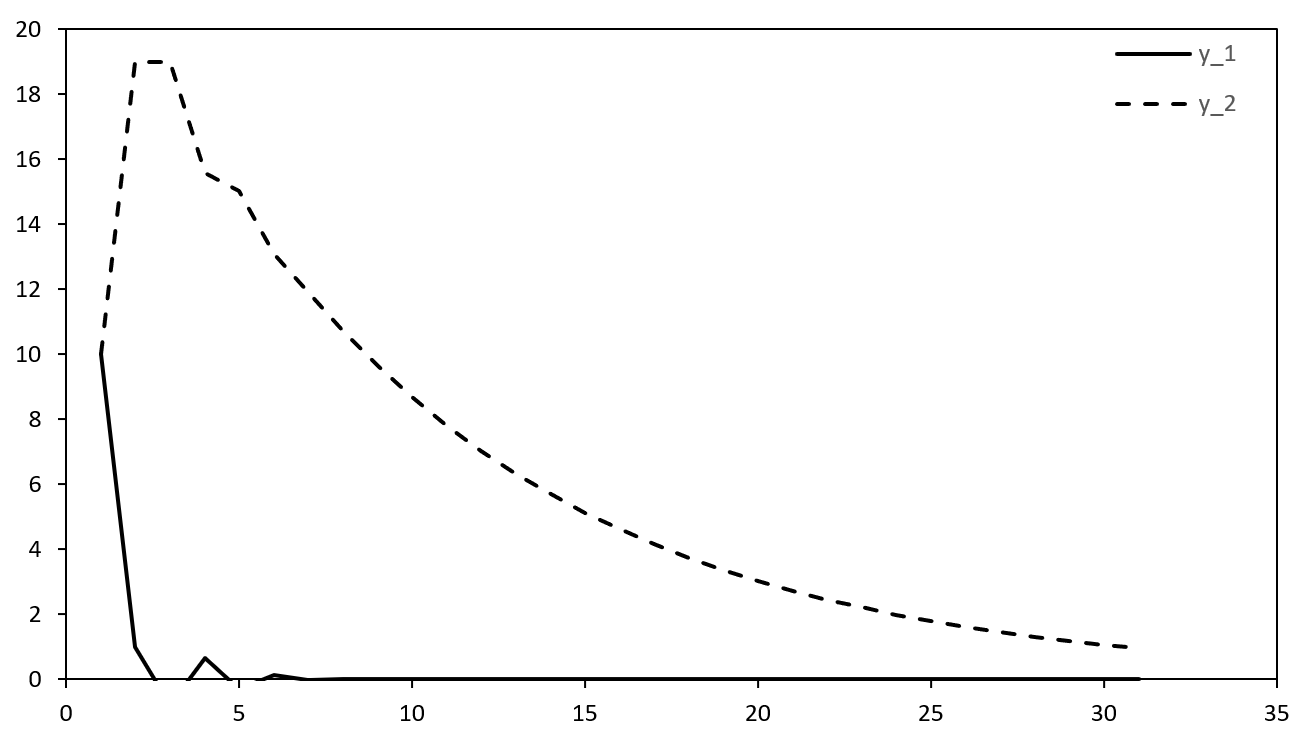
\includegraphics[width=12cm]{img/y2big_ac.png}
\caption{$y_2 > a/c$の場合}
\label{fig:y2>a/c}
\end{figure}

$y_2 < a/c$の場合は図\ref{fig:y2<a/c}のようになる。
\begin{figure}[H]
\centering
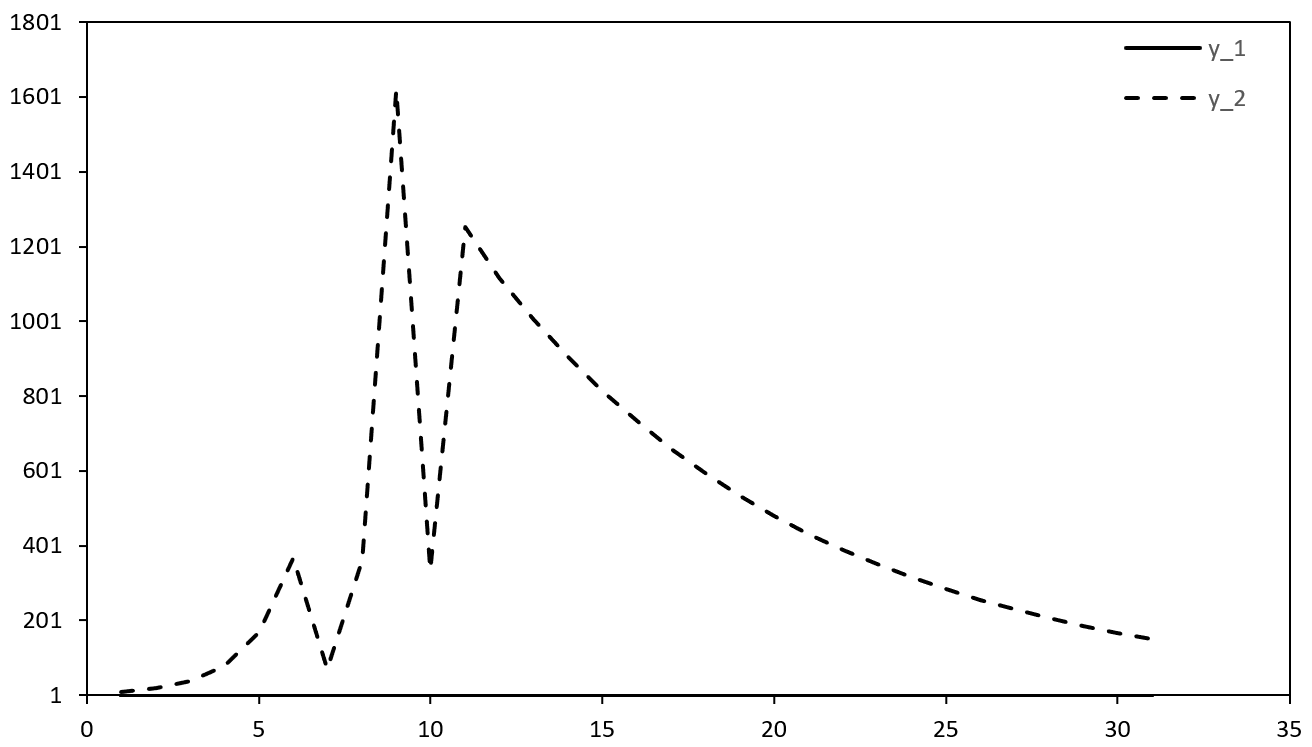
\includegraphics[width=12cm]{img/y2small_ac.png}
\caption{$y_2 < a/c$の場合}
\label{fig:y2<a/c}
\end{figure}

$y_1 > b/d$の場合は図\ref{fig:y1>b/d}のようになる。
\begin{figure}[H]
\centering
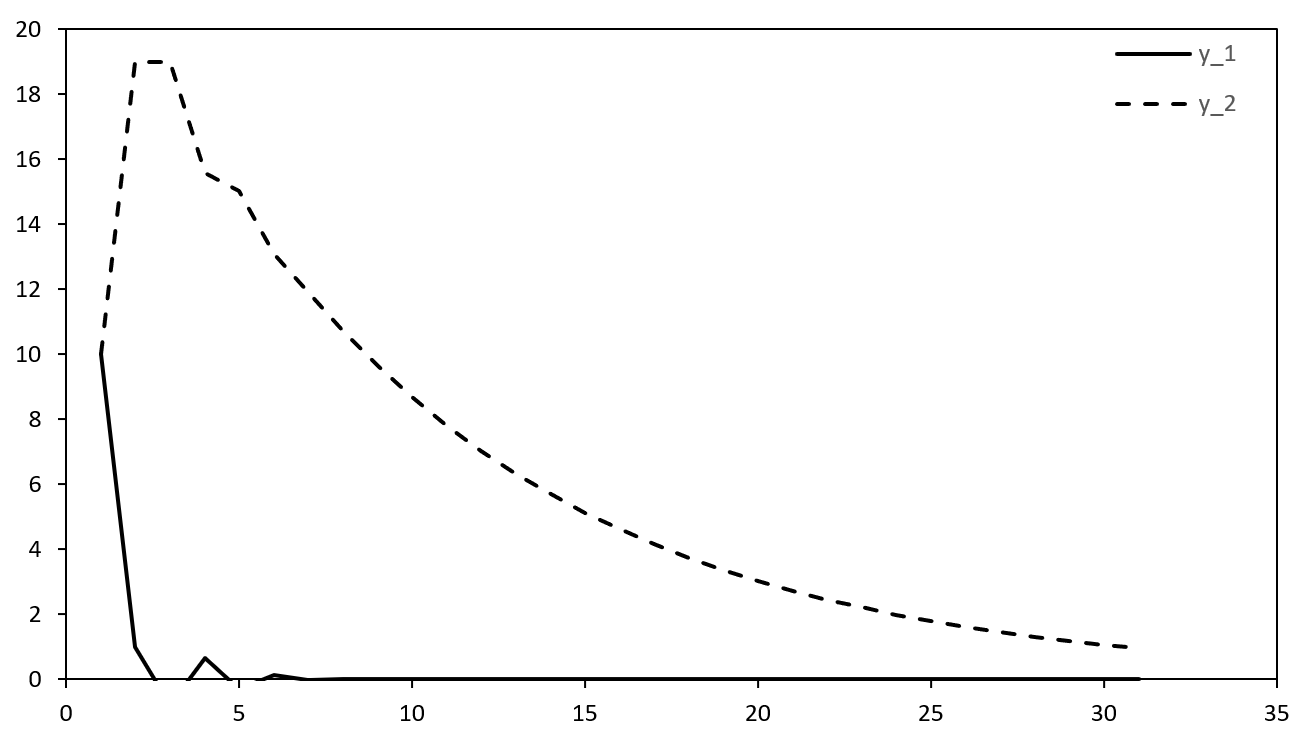
\includegraphics[width=12cm]{img/y2big_ac.png}
\caption{$y_1 > b/d$の場合}
\label{fig:y1>b/d}
\end{figure}

$y_1 < b/d$の場合は図\ref{fig:y1<b/d}のようになる。
\begin{figure}[H]
\centering
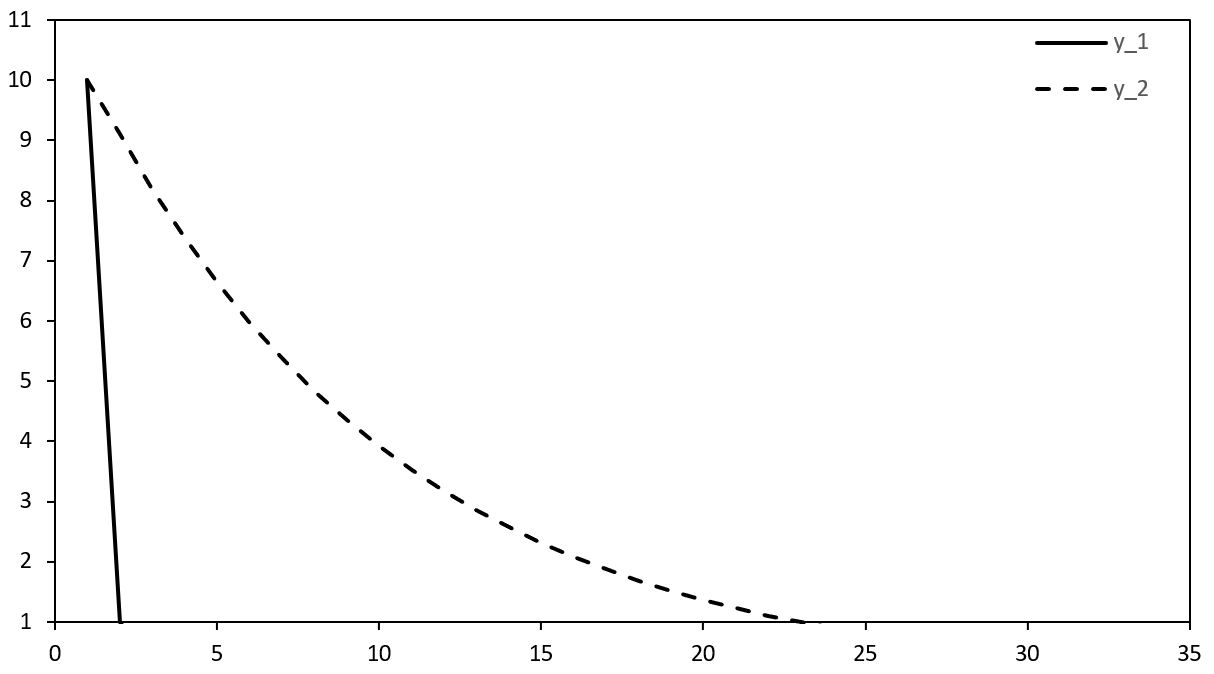
\includegraphics[width=12cm]{img/y1small_bd.png}
\caption{$y_1 < b/d$の場合}
\label{fig:y1<b/d}
\end{figure}

\section{課題7}
課題7では、式(\ref{eq:newton})に示す高階微分方程式のニュートンの運動方程式をオイラー法で解くプログラムを作成する。そして、$l=0$の場合に単振動することを確認する。今回は、$t=0, y=0, y'=0, m=1$とする。

\begin{equation}
\label{eq:newton}
	y''=\frac{-kx-ly'}{m}
\end{equation}

ここで、式(\ref{eq:newton})において、速度を表す従属変数vを導入して、$y'=v$とすれば

\begin{eqnarray}
\label{eq:newtonODEs}
	\left\{
		\begin{array}{l}
			v'=\frac{-kx-lv}{m}\\
			y'=v
		\end{array}
	\right.
\end{eqnarray}

という連立1階微分方程式が得られる。この式(\ref{eq:newtonODEs})は課題6と同じように解くことができる。

\subsection{作成したプログラム}
今回作成したプログラムをソースコード\ref{src:kadai7}に示す。

\lstinputlisting[caption=課題7のプログラム,label=src:kadai7]{src/kadai7.c}

このプログラムでは、刻み幅hは0.005とし、計算ステップ数を2000回に設定した。

\subsection{プログラムの実行結果}
実行結果を以下に示す。なお、出力される実行結果が多いため一部のみを掲載する。
\begin{oframed}
\verbatimtabinput[2]{result/kadai7.txt}
\end{oframed}

\subsection{考察}
出力された結果をグラフにすると図\ref{fig:kadai7}のようになる。これより、単振動していることがわかる。
\begin{figure}[H]
\centering
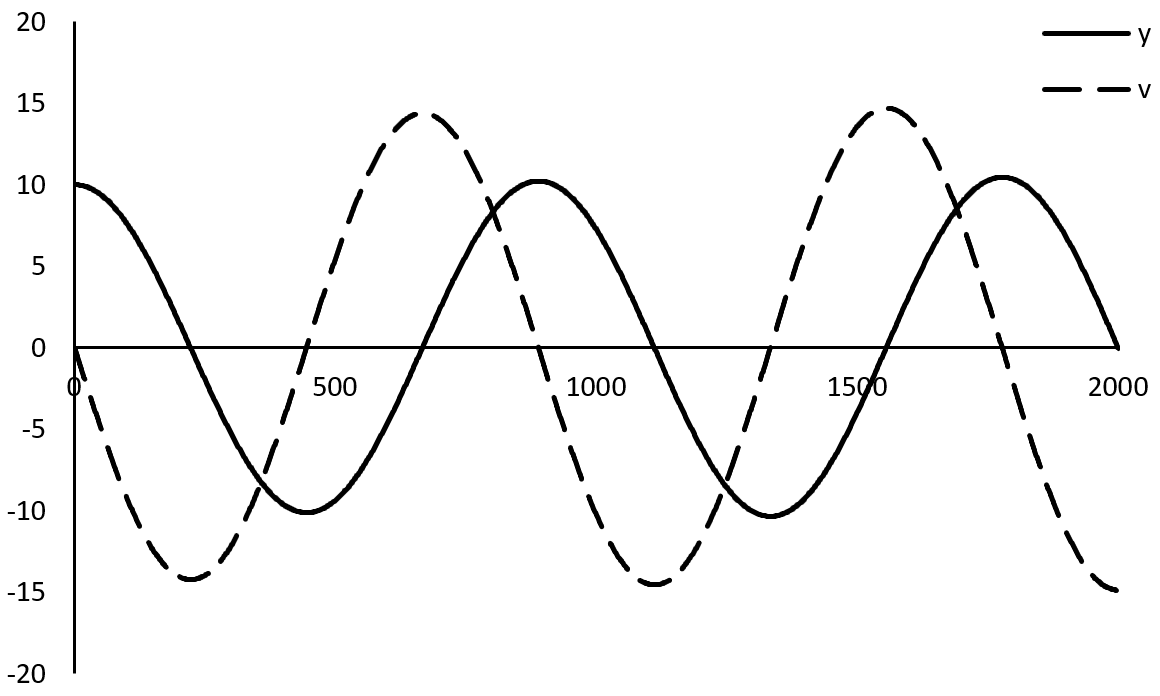
\includegraphics[width=12cm]{img/kadai7.png}
\caption{課題7の単振動の様子}
\label{fig:kadai7}
\end{figure}

また、kの値を4にした場合を図\ref{fig:kadai7_k}、lの値を4にした場合を図\ref{fig:kadai7_l}にそれぞれ示す。
\begin{figure}[H]
\centering
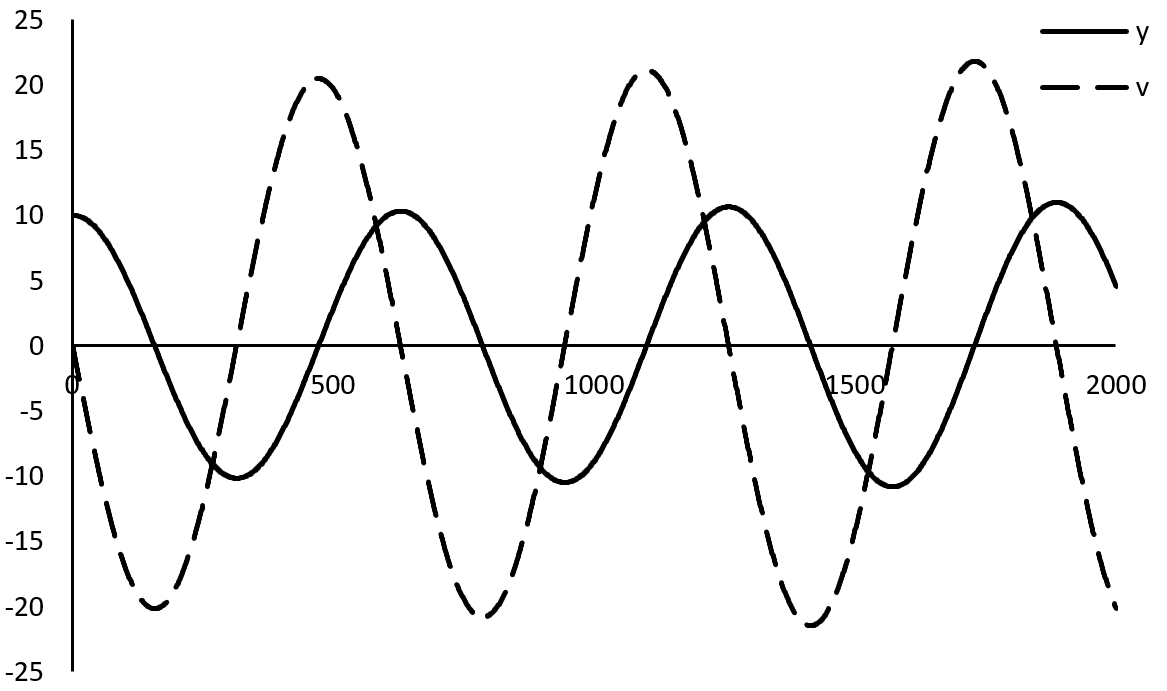
\includegraphics[width=12cm]{img/kadai7_k.png}
\caption{kの値が4の場合}
\label{fig:kadai7_k}
\end{figure}

これよりkの値は単振動の周期を決める事がわかる。

\begin{figure}[H]
\centering
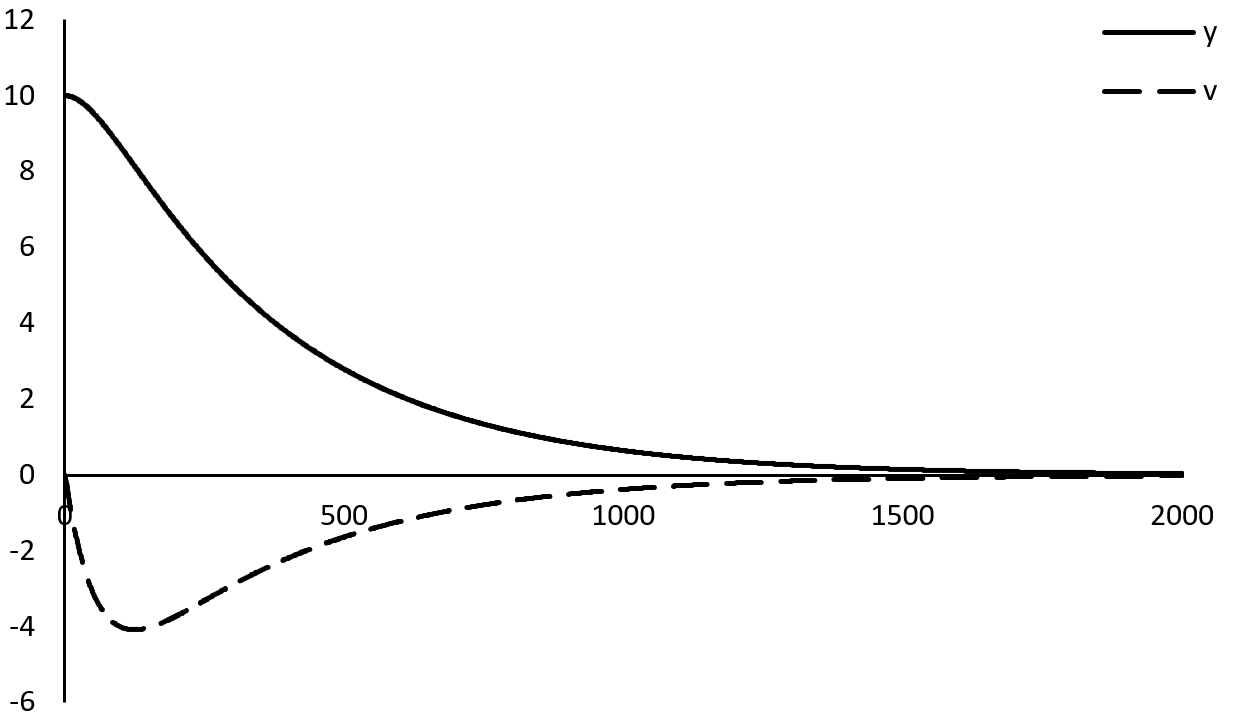
\includegraphics[width=12cm]{img/kadai7_l.png}
\caption{lの値が4の場合}
\label{fig:kadai7_l}
\end{figure}

lの値を大きくすると、単振動の振れ幅が小さくなることがわかる。


\section{課題8}
RLC共振回路の微分方程式
\begin{equation}
\label{eq:RLC}
	L\frac{d^2Q}{dt^2}+R\frac{dQ}{dt}+\frac{Q}{C}=0
\end{equation}
の式(\ref{eq:RLC})をホイン法によって解くプログラムを作成する。そして、R=0の場合に、単振動することを確認する。
ここで、初期条件は$t=0, Q=Q_0, dQ/dt=0$とする。また、パラメータは$R=1[k\Omega], C=0.3[nF], L=10[mH], Q_0=10[pC]$程度の値を用いる。

\begin{itembox}[l]{ホイン法}
\centering
	$x_{i+1}=x_i+h$\\
	$k_1=hf(x_i,y_i)$\\
	$k_2=hf(x_i+h,y_i+k_1)$\\
	$y_{i+1}=y_i+\frac{1}{2}(k_1+k_2)$
\end{itembox}

\subsection{作成したプログラム}
作成したプログラムをソースコード\ref{src:kadai8}に示す。

\lstinputlisting[caption=課題8のプログラム,label=src:kadai8]{src/kadai8.c}

ここで、ホイン法の刻み幅hは0.01で、計算ステップ数を2000回とする。

\subsection{プログラムの実行結果}
実行結果を以下に示す。なお、出力される結果が多いため一部のみを掲載する。
\begin{oframed}
\verbatimtabinput[2]{result/kadai8.txt}
\end{oframed}

\subsection{考察}
出力された結果をグラフにすると図\ref{fig:kadai8}のようになる。これより、単振動していることがわかる。
\begin{figure}[H]
\centering
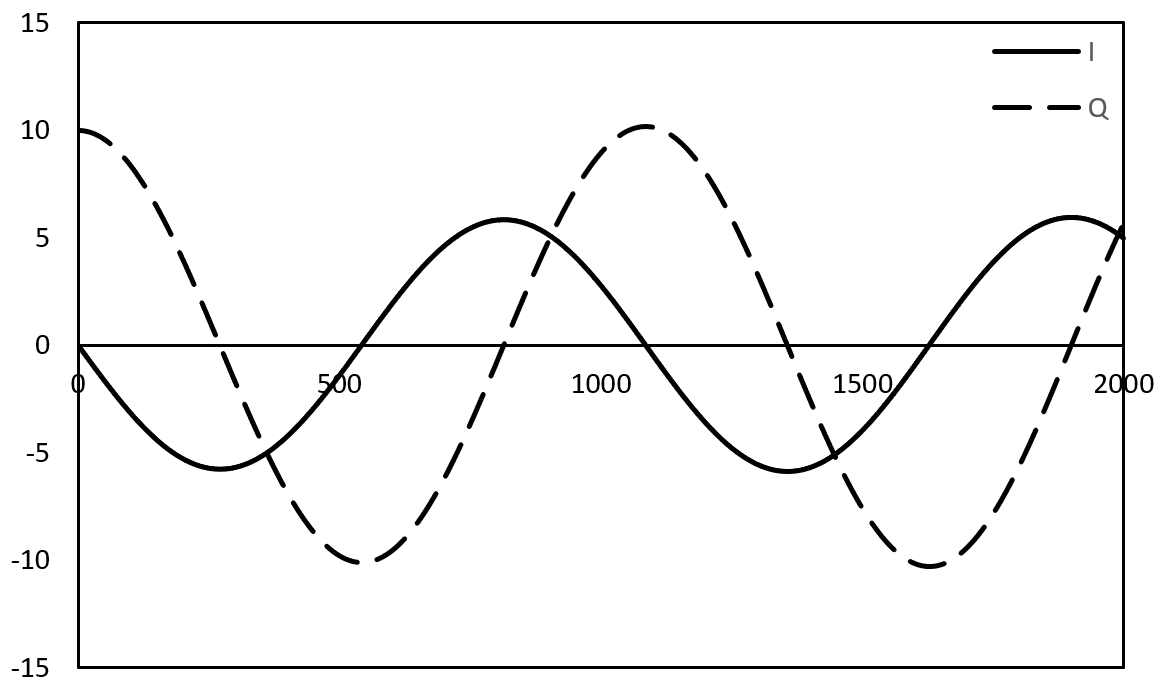
\includegraphics[width=12cm]{img/kadai8.png}
\caption{課題8の単振動の様子}
\label{fig:kadai8}
\end{figure}

次にRの値を$R=2\sqrt{L/C}$にしたときの様子を図\ref{fig:kadai8_R}に示す。
\begin{figure}[H]
\centering
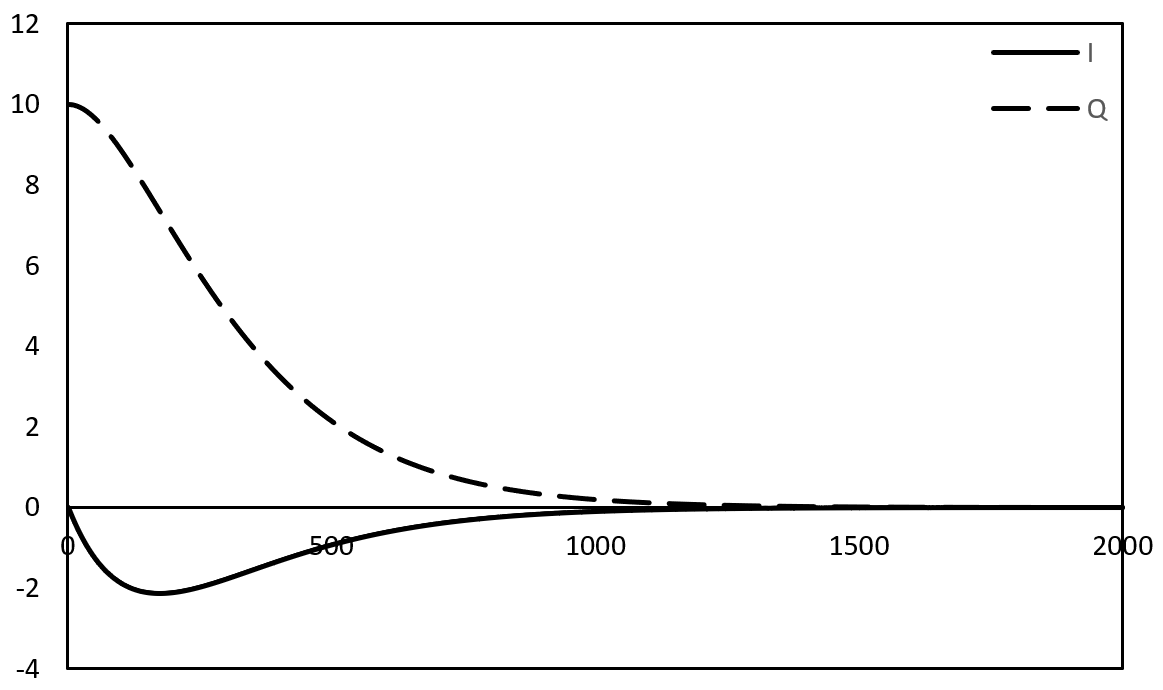
\includegraphics[width=12cm]{img/kadai8_R.png}
\caption{$R=2\sqrt{L/C}$の場合}
\label{fig:kadai8_R}
\end{figure}

これより、振動しなくなり、値が0に近づいていることがわかる。


\section{課題9}
課題9では式(\ref{eq:kadai9_2})(\ref{eq:kadai9_2})をホイン法で数値的に解くプログラムを作成する。
また、エネルギー保存則の式(\ref{eq:energy})が成り立つように刻み幅を設定する。なお、初期条件として、$t=0,x=0.1,y=0.0,v_x=0.0,v_y=0.1$とし、$q=m=1.0$とする。

\begin{eqnarray}
\label{eq:kadai9_2}
	\left\{
		\begin{array}{l}
			v_x'=\frac{q}{m}v_yB_0\\
			x'=v_x
		\end{array}
	\right.
\end{eqnarray}

\begin{eqnarray}
\label{eq:kadai9_3}
	\left\{
		\begin{array}{l}
			v_y'=-\frac{q}{m}v_xB_0\\
			y'=v_y
		\end{array}
	\right.
\end{eqnarray}

\begin{equation}
\label{eq:energy}
	v^2_x+v^2_y=constant
\end{equation}

\subsection{作成したプログラム}
作成したプログラムをソースコード\ref{src:kadai9}に示す。

\lstinputlisting[caption=課題9のプログラム,label=src:kadai9]{src/kadai9.c}

ここでは、刻み幅を0.005、計算ステップ数を500回としている。

\subsection{プログラムの実行結果}
実行結果を以下に示す。なお、出力される結果が多いため一部のみを掲載する。
\begin{oframed}
\verbatimtabinput[2]{result/kadai9.txt}
\end{oframed}
結果より、誤差はほとんど発生していないことがわかる。

\subsection{考察}
ここでは、磁場の値Bを1,5,10と変化させて粒子の運動がどのように変化するか考察する。
図\ref{fig:kadai9_B1},\ref{fig:kadai9_B5},\ref{fig:kadai9_B10}に変化させた時の様子を示す。

\begin{figure}[H]
\centering
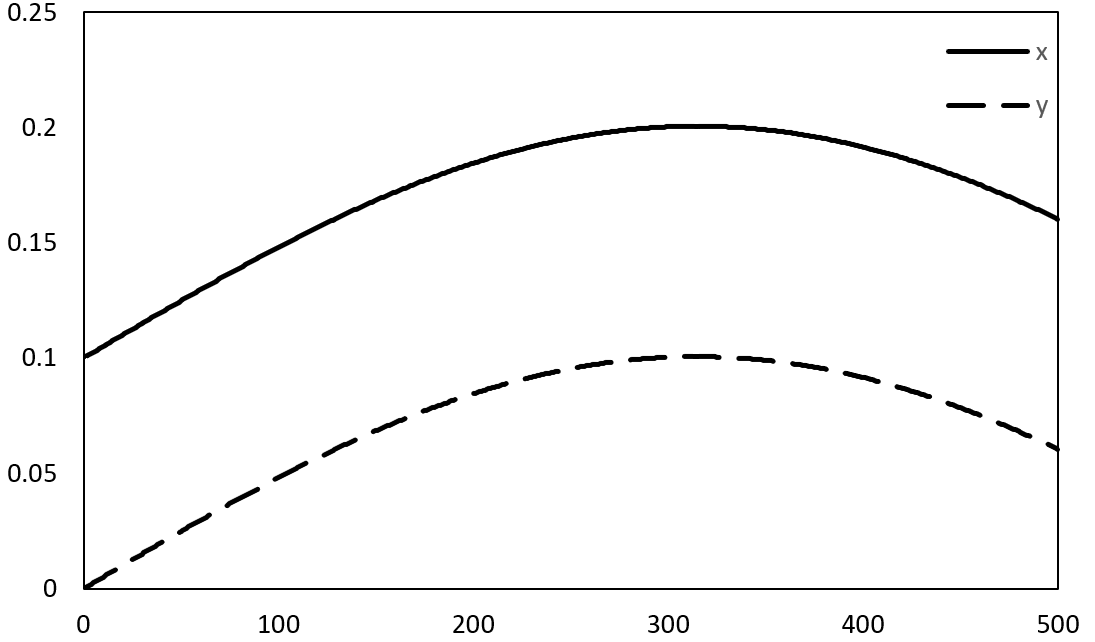
\includegraphics[width=12cm]{img/kadai9_B1.png}
\caption{$B=1$の場合}
\label{fig:kadai9_B1}
\end{figure}

\begin{figure}[H]
\centering
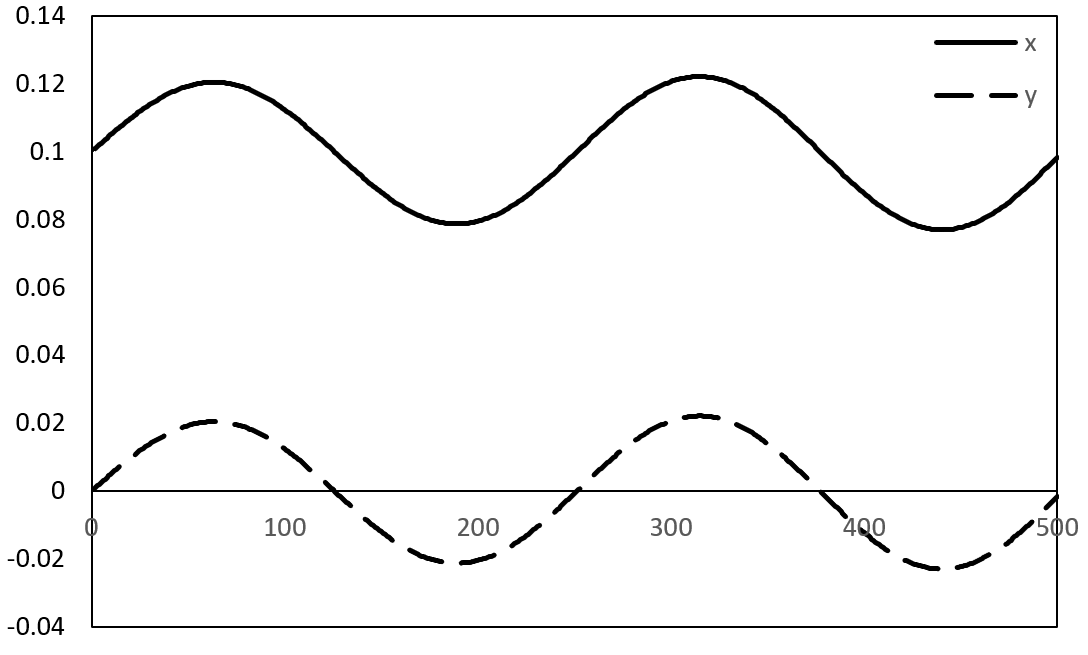
\includegraphics[width=12cm]{img/kadai9_B5.png}
\caption{$B=5$の場合}
\label{fig:kadai9_B5}
\end{figure}

\begin{figure}[H]
\centering
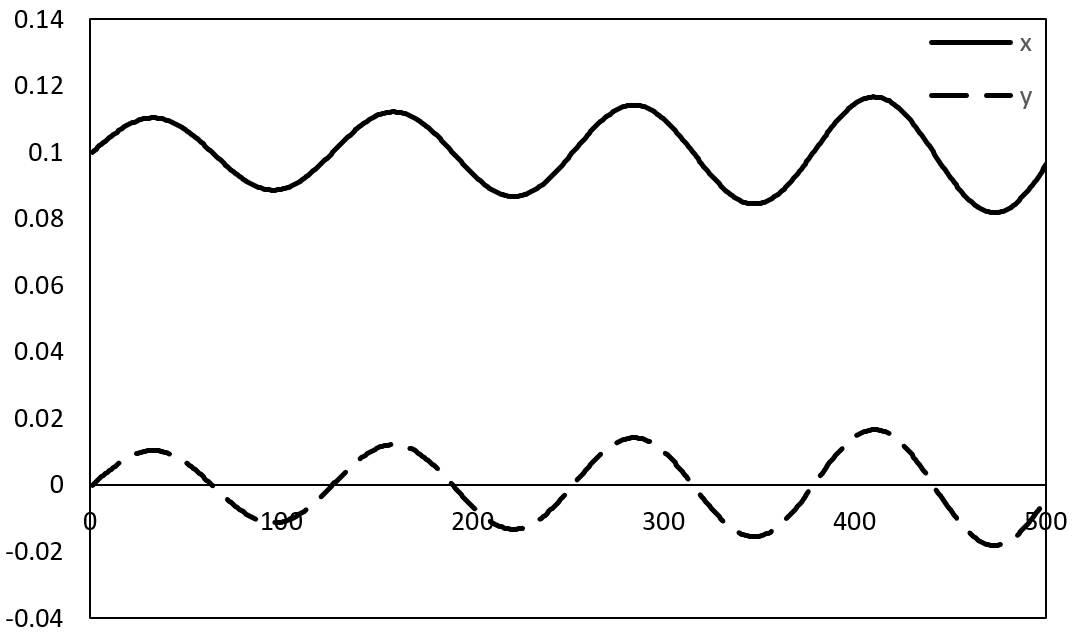
\includegraphics[width=12cm]{img/kadai9_B10.png}
\caption{$B=10$の場合}
\label{fig:kadai9_B10}
\end{figure}

Bの値を大きくすると振動の周期が大きくなることがわかる。

\section{課題10}
課題10では、課題9の式に式(\ref{eq:kadai10})が示す、電場から受ける力を追加し、粒子の運動がどうなるかを報告する。ここでは、$B=E=1.0$とし、初期条件は、$t=0.0のとき,x=0.1,y=0.0,z=0,0,v_x=0.0,v_y=0.1,v_z=0.0$とする。また、$q=m=1.0$とする。

\begin{eqnarray}
\label{eq:kadai10}
	\left\{
		\begin{array}{l}
			v_z'=\frac{q}{m}z\\
			z'=v_z
		\end{array}
	\right.
\end{eqnarray}

\subsection{作成したプログラム}
作成したプログラムをソースコード\ref{src:kadai10}に示す。

\lstinputlisting[caption=課題10のプログラム,label=src:kadai10]{src/kadai10.c}
ここでは、刻み幅を0.05とし、計算ステップ数を4000回としている。

\subsection{プログラムの実行結果}
実行結果を以下に示す。なお、出力される結果が多いため一部のみを掲載する。
\begin{oframed}
\verbatimtabinput[2]{result/kadai10.txt}
\end{oframed}


\subsection{考察}
出力された結果を3次元プロットしたものを図\ref{fig:kadai10}に示す。

\begin{figure}[H]
\centering
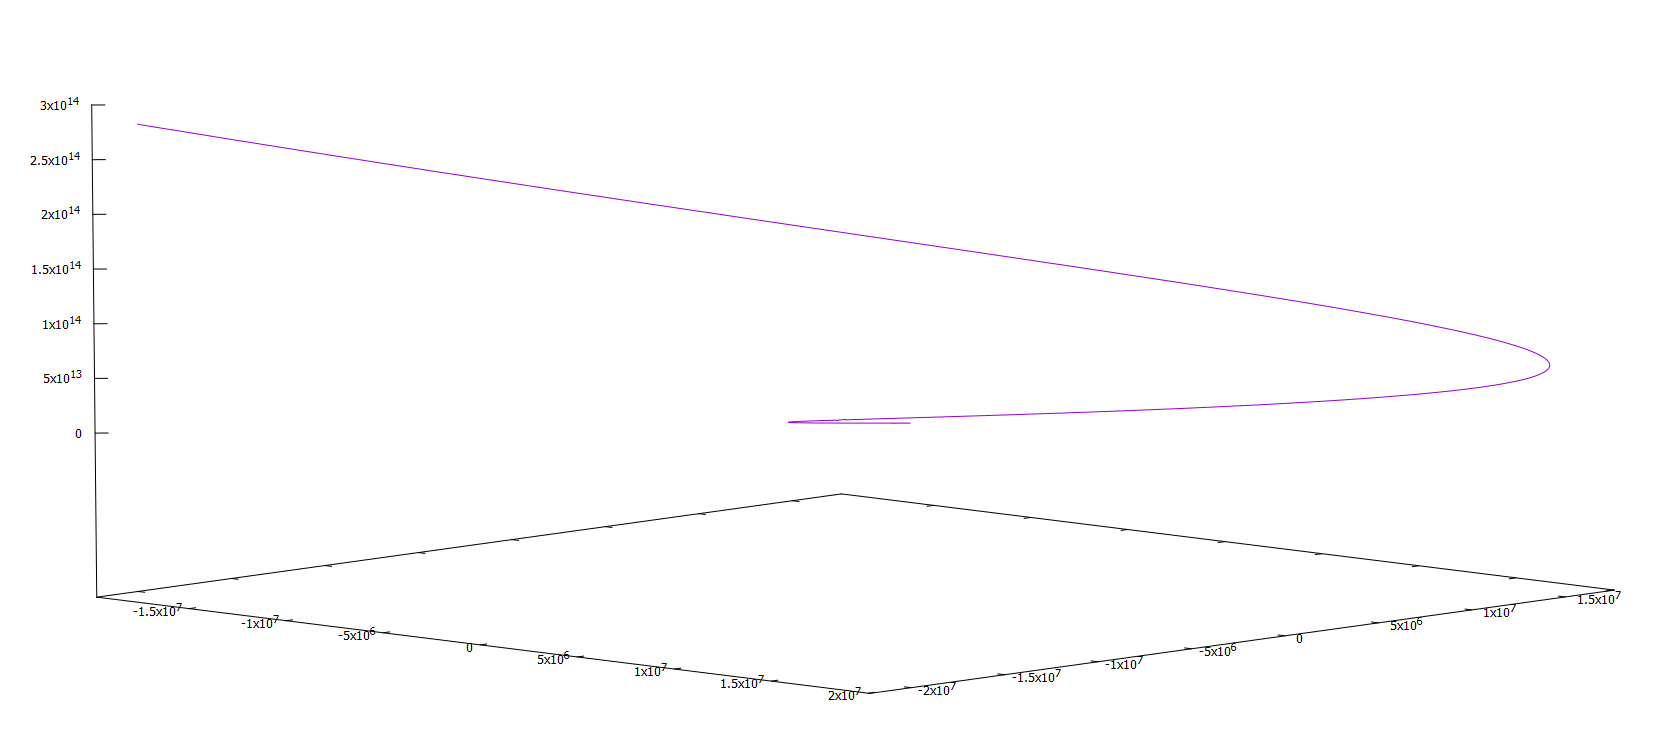
\includegraphics[width=12cm]{img/kadai10.png}
\caption{課題10の3次元プロット}
\label{fig:kadai10}
\end{figure}

これより、運動の振れ幅が大きく増加することがわかる。

\end{document}